\documentclass[
../../EiKI_Summary.tex,
]
{subfiles}
    
\externaldocument[ext:]{../../EiKI_Summary.tex}
% Set Graphics Path, so pictures load correctly
\graphicspath{{../../}}

\begin{document}
\section{Logic \& AI: Propositional Logic}
Search Algorithms only evaluate states, but do not have an ''understanding'' of the environment. This does mean, that a goal might not even be able to exist logically, but the search algorithms will still search for it.

\defc{Propositional Logic} aims to improve on that aspect.

\subsection{Logic}
Logic is the key behind any formal knowledge. It allows to filter neccessary information from a set of information and to draw conclusions. In AI, any representation of knowledge is based on logic.

\begin{defbox}
    [Knowledge Base (KB)]
    A knowledge base represents actual facts which exist in the real world. It is a central component of any knowledge-based agent. It is a collection of ''sentences'' in a formal language which describe the information related to the world.
\end{defbox}

\begin{defbox}
    [Inference Engine]
    The inference engine is responsible for inferring new knowledge from the knowledge base. It is a central component of any knowledge-based agent.
\end{defbox}

\begin{figure}
    [H]
    \centering
    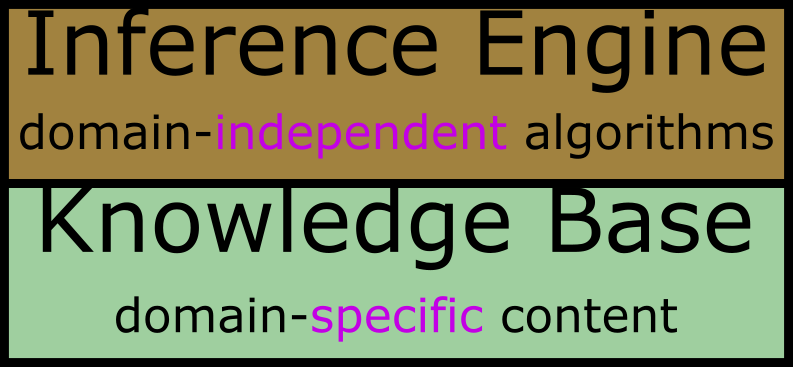
\includegraphics[width=0.4\textwidth]{Pics/06/Knowledge_Inference.png}
\end{figure}

\begin{defbox}
    [Knowledge-Based Agents]
    A knowledge-based agent is a type of \defc{intelligent agent} that uses a knowledge base and an inference engine to make decisions. 

    \begin{codebox*}
        \begin{algorithm}[H]
            \SetKwFunction{kbagent}{knowledge\_based\_agent}
            \SetKwFunction{tell}{tell}
            \SetKwFunction{ask}{ask}
            \SetKwFunction{makeperceptsentence}{make\_percept\_sentence}
            \SetKwFunction{makeactionquery}{make\_action\_query}

            kb; \tcp*[h]{The knowledge base}
            t; \tcp{counter, indicating time}
            \Fn{\kbagent{percept}}{
                \tell{kb, \makeperceptsentence{percept,t}}\;
                action = \ask{kb, \makeactionquery{t}}\;
                \tell{kb, \makeperceptsentence{action,t}}
                t++\;
                \KwRet action
            }
        \end{algorithm}
    \end{codebox*}

    \begin{itemize}
        \item Represent states, actions\dots
        \item Incorporate new percepts and update knowledge base
        \item Deduce properties of the world and make decisions / actions
    \end{itemize}
\end{defbox}

\newpage
\subsection{Syntax}
A sentence in propositional logic follows the \defc{Backus-Naur Form (BNF)}:

\begin{tabular}{r l l}
    \defc{Symbol:}   & P, Q, R,\dots & Descriptor of a sentence\\
    \defc{Sentence:} & True | False | Symbol | & Logical implication of a sentence\\
    & $\neg$(Sentence) | &\\
    & (Sentence $\land$ Sentence) | &\\
    & (Sentence $\lor$ Sentence) | &\\
    & (Sentence $\Rightarrow$ Sentence) &\\
\end{tabular}

\subsection{Semantics}
\defc{Interpretation} specifies which symbols are true and which are false. Given a interpretation it should be possible to evaluate a sentence. 

A truth table defines semantics of operators:
\[
\begin{array}{|c|c|c|c|c|c|}
\hline
a & b & \neg a & a \land b & a \lor b & a \Rightarrow b \\
\hline
\text{false} & \text{false} & \text{true} & \text{false} & \text{false} & \text{true} \\
\text{false} & \text{true} & \text{true} & \text{false} & \text{true} & \text{true} \\
\text{true} & \text{false} & \text{false} & \text{false} & \text{true} & \text{false} \\
\text{true} & \text{true} & \text{false} & \text{true} & \text{true} & \text{true} \\
\hline
\end{array}
\]

\subsection{Tautology}
A tautolgy is a sentence that is true for all possible interpretations.
\[
\begin{array}{|c|c|c|c|c|}
\hline
P & Q & P \lor Q & \neg P \land \neg Q & \defc{(P \lor Q) \lor (\neg P \land \neg Q)} \\
\hline\hline
\text{false} & \text{false} & \text{false} & \text{true} & \text{true} \\
\text{false} & \text{true} & \text{true} & \text{false} & \text{true} \\
\text{true} & \text{false} & \text{true} & \text{false} & \text{true} \\
\text{true} & \text{true} & \text{true} & \text{false} & \text{true} \\
\hline
\end{array}
\]


\subsection{Logical Equivalence}
Two sentences are \defc{logically equivalent} if they have the same truth value for every setting of their propositional variables.

\[
\begin{array}{|c|c|c|c|}
\hline
P & Q & \defc{P\lor Q} & \defc{\neg (\neg P\land \neg Q)} \\
\hline\hline
\text{false} & \text{false} & \text{false} & \text{false} \\
\text{false} & \text{true} & \text{true} & \text{true} \\
\text{true} & \text{false} & \text{true} & \text{true} \\
\text{true} & \text{true} & \text{true} & \text{true} \\
\hline
\end{array}
\]

\begin{center}	
    \begin{tabular}{|c|c|}
        \hline
        \textbf{Logical Law} & \textbf{Equivalence} \\
        \hline\hline
        Commutativity & $(a \lor b) \equiv (b \lor a)$ \\
        & $(a \land b) \equiv (b \land a)$ \\
        \hline
        Associativity & $((a \land b) \land c) \equiv (a \land (b \land c))$ \\
        & $((a \lor b) \lor c) \equiv (a \lor (b \lor c))$ \\
        \hline
        Double Negation Elimination & $\lnot(\lnot a) \equiv a$ \\
        \hline
        Contraposition & $(a \Rightarrow b) \equiv (\lnot b \Rightarrow \lnot a)$ \\
        \hline
        Implication Elimination & $(a \Rightarrow b) \equiv (\lnot a \lor b)$ \\
        \hline
        De Morgan's Laws & $\lnot(a \land b) \equiv (\lnot a \lor \lnot b)$ \\
        & $\lnot(a \lor b) \equiv (\lnot a \land \lnot b)$ \\
        \hline
        Distributivity & $(a \land (b \lor c)) \equiv ((a \land b) \lor (a \land c))$ \\
        & $(a \lor (b \land c)) \equiv ((a \lor b) \land (a \lor c))$ \\
        \hline
    \end{tabular}
\end{center}

\subsection{Inference / Entailment}
A sentence is \defc{entailed} by the knowledge base if, for every setting of the propositional variables, for which knowledge base is true, the sentence is also true.

Assume 2 sentences, $A$ and $A \Rightarrow B$:

\begin{center}
	\begin{tabular}{|c|c|c|}
        \hline
        A & B & Knowledge base \\
        \hline\hline
        false & false & false \\
        false & true & false \\
        true & false & false \\
        true & true & true \\
        \hline
    \end{tabular}
\end{center}

To find out whether a sentence $A$ is entailed by knowledge base as simple algorithm can be used:

\textbf{Basic Idea:}
\begin{enumerate}
    \item Go through all possible setting of the propositional variables
    \item If knowledge base is true and $A$ is false $\Rightarrow$ return false
    \item Else $\Rightarrow$ return true
\end{enumerate}

\textbf{Problem:}
Not very efficient: The number of setting increases with $2^{\text{\# propositional variables}}$

\subsubsection{Principle of Non-Contradiction}
\begin{defbox*}
    \begin{center}
	''A cannot be $\neg$ A''
    \end{center}

    Two contradictionary statements cannot be true at the same time, as that would mean that anything could be true.
\end{defbox*}

\textbf{Example:}

PetIsABird $\Rightarrow$ PetCanFly\\
PetIsAPenguin $\Rightarrow$ PetIsABird\\
PetIsAPenguin $\Rightarrow$ $\neg$(PetCanFly)\\
PetIsAPenguin

This would imply that a penguin can both fly and not fly. If you would work with this contradictionary predicate it could imply anything like:

PetCanFly $\lor$ MoonMadeOfCheese $\equiv$ True

\subsection{Conjunctive Normal Form (CNF)}
The CNF is a way to write any knowledge base as a single formula:

\begin{defbox}
    [CNF Formula]
    \begin{center}
        $(\dots\lor\dots\lor\dots) \land (\dots\lor\dots\lor\dots) \land \dots$
    \end{center}
    \begin{itemize}
        \item Can be a symbol x or $\neg$(x) (\defc{Literals})
        \item Multiple fats in knowledge base are ''AND''ed together
    \end{itemize}
\end{defbox}

\textbf{Example:}
RoommateWet $\Rightarrow$ (RoommateWetOfRain $\lor$ RoommateWetOfSprinklers)\\
becomes\\
($\neg$(RoommateWet) $\lor$ RoommateWetOfRain $\lor$ RoommateWetOfSprinklers)

\subsection{Modus Ponens}
Modus Ponens allows to form new sentences from existing ones:

Assume two sentences, $A$ and $A \Rightarrow B$: From this we can conclude the new sentence $B$.

\subsubsection{Unit Resolution}
Assume the sentences $l_1 \lor l_2 \lor \dots \lor l_k$ and $\neg(l_i)$. 

From this we can conclude the new sentence: $l_1 \lor l_2 \lor \dots \lor l_{i-1} \lor l_{i+1} \lor \dots \lor l_k$

\subsubsection{General Resolution}
Assume two sentences $l_1 \lor l_2 \lor \dots \lor l_k$ and $m_1 \lor m_2 \lor \dots \lor m_n$ where for some $i,j$ $l_i = \neg(m_j)$. 

From this we can conclude the new sentence: $l_1 \lor l_2 \lor \dots \lor l_{i-1} \lor l_{i+1} \lor \dots \lor l_k \lor m_1 \lor m_2 \lor \dots \lor m_{j-1} \lor m_{j+1} \lor \dots \lor m_n$ 

The same literal may appear multiple times; these need to be removed.

\subsection{Resolution}
\begin{defbox}
    [Satisfiable]
    There exists a model that makes the modified knowledge base true, i.e., the modified knowledge base is consistent.
\end{defbox}

To see if a knowledge base is satisfiable, one can use a resolution algorithm.

\subsubsection{Resolution Algorithm}
\textbf{Basic Idea:}
CNF formula for modified knowledge base is satisfiable if and only if sentence $A$ is \defc{not entailed}.
So to see if a sentence $A$ is entailed we can simply add $\neg$A to the knowledge base and see if it becomes inconsistent.

\begin{enumerate}
    \item \defc{Find} two clauses with complementary literals
    \item \defc{Apply} resolution
    \item \defc{Add} resulting clause (if not already there)
    \item \defc{Test}, if it results in the empty clause $\rightarrow$ formula is not satisfiable 
\end{enumerate}

\subsubsection*{Special Case: Horn Clauses}
\begin{defbox}
    [Horn Clauses]
    Horn clauses are implications with only positive (no negations) literals:

    \begin{center}
        $X_1 \land X_2 \land X_4 \Rightarrow X_3 \land X_6$\\
        True $\Rightarrow X_1$
    \end{center}
\end{defbox}

To find out whether a literal $X_j$ is entailed:
\begin{enumerate}
    \item Start from known imlications as far as possible
    \item If $X_j$ is reachable it is entailed
\end{enumerate}

To increase efficiency of this approach we can maintain a count of how many implications are already known to reduce the neccessary computations.

\subsection{Limitations of Propositional Logic}
\begin{itemize}
    \item No notion of objects or relations: 
    \begin{itemize}
        \item Identifiers are merely suggestive, it does not neccessarily mean that the implied objects and relations actually exist or are real.
        \item To this end, every identifier might as well be a single letter $A,B\dots$
    \end{itemize}
\end{itemize}
\end{document}